Let 
% 
\begin{align}
\frac{3x-4}{2} = \frac{x+1}{4}-1 + s,  \quad s \geq 0
\end{align}
Then, 
\begin{align}
5x -5 -4s = 0 
\\
\implies x=1+\frac{4s}{5}
\\
\implies x \geq 1
\end{align}

The following code marks the solution of inequality on numberline as shown in figure \ref{fig:3.11.3_ineq_py}
\begin{lstlisting}
codes/line/ineq/ineq.py
\end{lstlisting}
\begin{figure}[!ht]
\centering
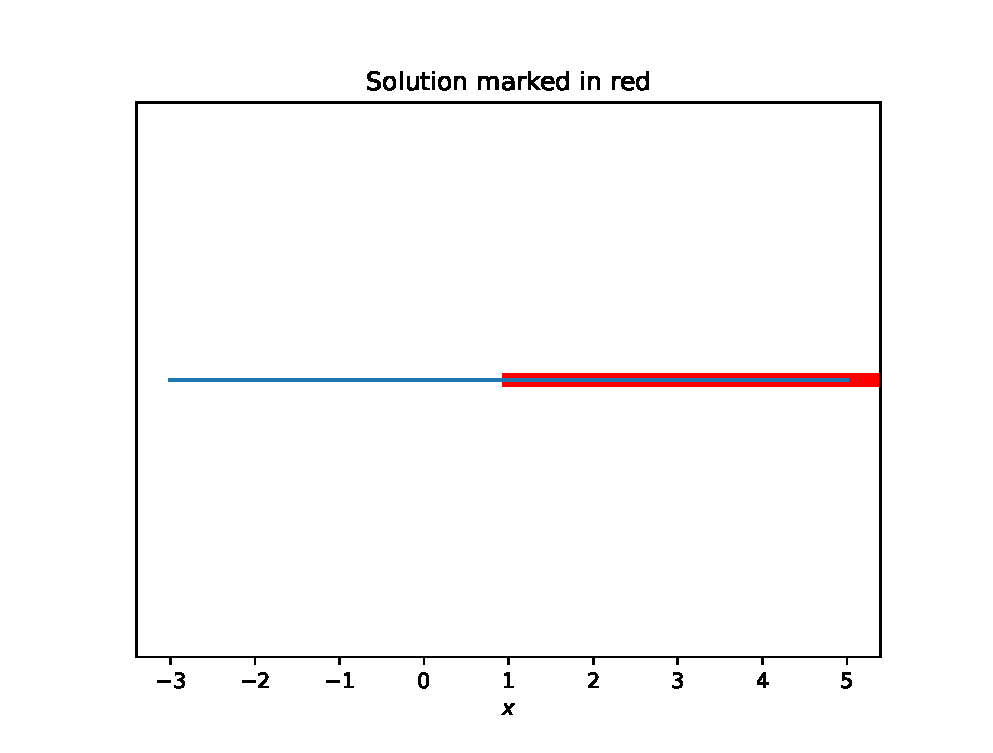
\includegraphics[width=\columnwidth]{./solutions/3/codes/line/ineq/pyfigs/ineq.eps}
\caption{Solution of the inequality}
\label{fig:3.11.3_ineq_py}
\end{figure}

